\documentclass[a4paper,12pt]{extarticle}
\usepackage[table,xcdraw]{xcolor}
\usepackage{pgfplots}
\usepackage[unicode, pdftex]{hyperref}
\usepackage[T2A]{fontenc}
\usepackage[utf8]{inputenc}
\usepackage[english,russian]{babel}
\usepackage{amsmath,amsfonts,amsthm, mathtools}
\usepackage{amssymb}
\usepackage{graphicx}
\graphicspath{{images/}}
\usepackage{wrapfig}
\usepackage{floatrow}
\usepackage{setspace}
\usepackage[headings]{fancyhdr}
%\usepackage[margin=10pt,font={small,stretch=0,9},labelfont=bf,labelsep=period,
%justification=centerlast]{caption}
\usepackage{array,tabularx,tabulary,booktabs}
\RequirePackage{multirow}
\RequirePackage{multicol}
\RequirePackage{longtable}
\usepackage{indentfirst}
\usepackage{hyperref}
\usepackage{icomma}
\newcommand*{\hm}[1]{#1\nobreak\discretionary{}
	{\hbox{$\mathsurround=0pt #1$}}{}}
%\usepackage{soulutf8}
\usepackage{etoolbox}
\usepackage{geometry}
\geometry{top=20mm}
\geometry{bottom=20mm}
\geometry{left=20mm}
\geometry{right=20mm}
\DeclareMathOperator{\sgn}{\mathop{sgn}}
\usepackage[OT1]{fontenc}
\usepackage{amsmath}
\usepackage{amsfonts}
\usepackage{amssymb}
%\usepackage{wasysym}
\usepackage{wrapfig}
%\usepackage{physics}
%\usepackage[normalem]{ulem}
\graphicspath{{images/}}
\DeclareGraphicsExtensions{.png,.jpg,.jpeg}
\usepackage{indentfirst}
\usepackage[T2A]{fontenc}
\usepackage{subfigure}
\usepackage{fancyhdr}
%\usepackage{caption}

\usepackage{tabularx}
\usepackage{floatrow}
\usepackage{multicol}
\usepackage{lastpage}


% Настройка отчёркиваний и нумерации
% \usepackage{fancyhdr}
% \pagestyle{fancy}
% \fancyhf{}

% \renewcommand{\headrulewidth}{0.5pt}
% \renewcommand{\footrulewidth}{0.5pt}

\title{Лабораторная работа №3.2.5\\
       <<Свободные и вынужденные колебания в электрическом контуре>>}
\author{Балдин Виктор}

\begin{document}

\maketitle

\section{Введение}
\textit{Свободные колебания} -- колебания, происходящие за счёт энергии заранее запасённой в системе (в процессе колебаний энергия в систему не попадает). Обозначим как $\gamma = \frac{R}{2L}$ -- коэффициент затухания, тогда возникает классификация <<режимов>> колебаний в контуре:
\begin{enumerate}
    \item \text{Затухающие ($0 < \gamma < \omega_0$)}.
    \item \text{Критический режим ($\gamma = \omega_0$)} .
    \item \text{Апериодический режим ($\gamma > \omega_0$)}.
\end{enumerate}

\textit{Критическое сопротивление} -- сопротивление цепи, при котором происходит переход на апериодический режим
\textit{Вынужденные колебания} -- колебания, происходящие за счёт действия периодической внешней силы.
В данной работе мы будем изучать различные свойства и параметры как свободных, так и вынужденных колебаний в RLC контуре.


\textbf{Цели работы:}
\begin{enumerate}
    \item Изучение свободных колебаний в RLC контуре:
    \begin{itemize}
        \item Сравнить зависимость периода колебаний цепи от ёмкости с теоретической.
        \item Определение зависимости логарифмического декремента затухания от сопротивления цепи.
        \item Определение критического сопротивления контура.
    \end{itemize}
    \item Изучение вынужденных колебаний в RLC контуре:
    \begin{itemize}
        \item Построение резонансных кривых колебательного контура: АЧХ и ФЧХ.
        \item Определение декремента затухания колебательного контура по нарастанию колебаний и по их затуханию.
        \item Проанализировать картину биений.
    \end{itemize}
    \item Определение добротности контура различными способами.
\end{enumerate}

\newpage
\section{Теоретическая часть}
\begin{wrapfigure}[14]{r}{0.4\linewidth}
	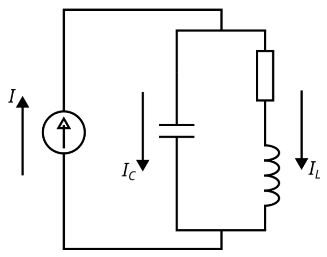
\includegraphics[width=\linewidth]{shem.png}
	\caption{Описываемый RLC контур}
\end{wrapfigure}
\noindent Для RLC контура (рис. 1) применим 2 правило Кирхгофа:
\begin{equation}
    RI + U_C + L\frac{dI}{dt} = 0.
\end{equation}
Подставив в уравнение (1) выражение для тока через 1-ое правило Кирхгофа, и разделив обе части уравнения на $CL$, получим:
\begin{equation}
    \frac{d^2U_C}{dt^2} + \frac{R}{L} \frac{dU_C}{dt} + \frac{U_C}{CL}.
\end{equation}
Произведём замены $\gamma = \frac{R}{2L}$ -- коэффициент затухания, $\omega_0^2 = \frac{1}{LC}$ -- собственная круговая частота, $T_0 = \frac{2\pi}{\omega_0} = 2\pi \sqrt{LC}$ -- период собственных колебаний. Тогда уравнение (2) примет вид:
\begin{equation}
    \ddot{U_C} + 2 \gamma \dot{U_C} + \omega_0^2U_C = 0,
\end{equation}
где точкой обозначено дифференцирование по времени. Будем искать решение данного дифференциального уравнения в классе функций следующего вида:
$$U_C(t) = U(t)e^{- \gamma t}.$$
Получим:
\begin{equation}
    \ddot{U} + \omega_1^2 U = 0,
\end{equation}
где
\begin{equation}
    \omega_1^2 = \omega_0^2-\gamma^2
\end{equation}
Для случая $\gamma < \omega_0$ в силу того, что $\omega_1 > 0$, получим:
\begin{equation}
    U_C(t) = U_0 \cdot e^{-\gamma t} \text{cos}(\omega_1 t + \varphi_0).
\end{equation}
Для получения фазовой траектории представим формулу (6) в другом виде:
\begin{equation}
    U_C(t) = e^{-\gamma t}(a \text{cos} \omega_1 t + b \text{sin} \omega_1 t),
\end{equation}
где $a$ и $b$ получаются по формулам:
$$a = U_0 \text{cos} \varphi_0, \qquad b = - U_0 \text{sin} \varphi_0.$$
В более удобном виде запишем выражения для напряжения на конденсаторе и токе через катушку:
\begin{equation}
    U_C (t) = U_{C0} \cdot e^{-\gamma t} (\text{cos} \omega_1 t + \frac{\gamma}{\omega_1} \text{sin} \omega_1 t),
\end{equation}
\begin{equation}
    I(t) = C\dot{U_C}= - \frac{U_{C0}}{\rho} \frac{\omega_0}{\omega_1} e^{-\gamma t} \text{sin} \omega_1 t.
\end{equation}
Введём некоторые характеристики колебательного движения:
\begin{equation}
    \tau = \frac{1}{\gamma} = \frac{2L}{R},
\end{equation}
где $\tau$ -- время затухания (время, за которое амплитуда колебаний уменьшается в $e$ раз).
\begin{equation}
    \Theta = \text{ln} \frac{U_k}{U_{k+1}} = \gamma T_1 = \frac{1}{N_\tau} = \frac{1}{n} \text{ln} \frac{U_k}{U_{k+n}},
\end{equation}
где $\Theta$ -- логарифмический декремент затухания, $U_k$ и $U_{k+1}$ -- два последовательных максимальных отклонения величины в одну сторону, $N_\tau$ -- число полных колебаний за время затухания $\tau$.

Теперь рассмотрим случай \textit{вынужденных колебаний} под действием внешней внешнего синусоидального источника. Для этого воспользуемся методом \textit{комплексных амплитуд} для схемы на рисунке (рис. 1):
\begin{equation}
    \ddot{I} + 2 \gamma \dot{I} + \omega^2 I = - \varepsilon \frac{\Omega}{L} e^{i\Omega t}.
\end{equation}
Решая данное дифференциальное уравнение получим решение:
\begin{equation}
    I = B\cdot e^{-\gamma t} \text{sin}(\omega t - \Theta) + \frac{\varepsilon_0 \Omega}{L \phi_0} \text{sin} (\Omega t - \varphi).
\end{equation}
Нетрудно видеть, что частота резонанса будет определяться формулой:
\begin{equation}
    \omega_0 = \frac{1}{2 \pi \sqrt{LC}}.
\end{equation}

Способы измерения \textbf{добротности}:
\begin{enumerate}
    \item с помощью потери амплитуды свободных колебаний:
    \begin{equation}
        Q = \frac{1}{n} \text{ln}\frac{U_k}{U_{k+n}},
    \end{equation}
    \item с помощью амплитуды резонанса можно получить добротность (в координатах $U_C/U_0$, где $U_0$ -- амплитуда колебаний напряжения источника, от частоты генератора). Отсюда нетрудно определить декремент затухания $\gamma = \frac{\omega_0}{2Q}$,
    \item с помощью среза АЧХ на уровне 0.7 от максимальной амплитуды, тогда <<дисперсия>> ($\Delta \Omega$) будет численно равна коэффициенту $\gamma$, то есть $Q = \frac{\nu_0}{2 \Delta \Omega}$.
    \item с помощью нарастания амплитуд в вынужденных колебаниях:
    \begin{equation}
        Q = \frac{\omega_0 n}{2\text{ln} \frac{U_0 - U_k}{U_0 - U_{k+n}}}.
    \end{equation}
\end{enumerate}

\newpage
\section{Экспериментальная установка}
Схема установки для изучения собственных колебаний представлена на рисунке (2), по ходу работы она будет претерпевать некоторые изменения, связанные со съёмом сигнала с различных её частей, что на принцип работы не повлияет, основным же изменением будет смена работы генератора сигналов, соответствующий режим будет описан в практической части, при переходе на него. Пунктиром показана схема подключения при снятия данных о колебаниях в фазовой плоскости, на рисунке (3) изображена схема установки для исследования АЧХ, ФЧХ и наблюдения биений.

\begin{figure}[h!]
    \centering
    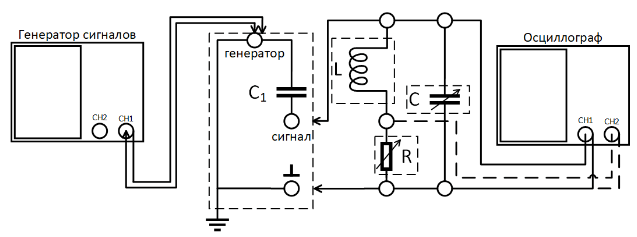
\includegraphics[width=0.8\linewidth]{ustan1.png}
    \caption{Схема установки для изучения собственных колебаний}
\end{figure}

\begin{figure}[h!]
    \centering
    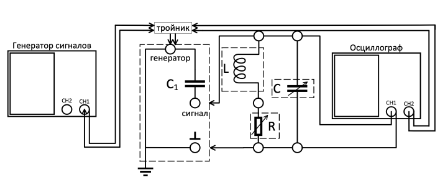
\includegraphics[width=0.8\linewidth]{ustan2.png}
    \caption{Схема установки для изучения вынужденных колебаний и биений}
\end{figure}

Красным прямоугольником выделен колебательный контур, \textit{<<состояния>>} элементов так же будут описаны в практической части. Конденсатор ($C_1$) между генератором сигналов и колебательным контуром служит для того, чтобы импеданс генератора был много меньше импеданса колебательного контура и не влиял на процессы, происходящие в контуре.

\newpage
\section{Практическая часть}
Соберём установку с рисунка 2, выставим $L =$ 100 мГн, $R =$ 0 Ом, $C =$ 0 мкФ, однако контур сам по себе обладает некоторым $C_0$, благодаря которому свободные колебания могут быть реализованы, а их затухание будет обеспечено активным сопротивлением катушки индуктивности. Переведём генератор сигналов в режим <<Pulse>>, установим частоту 100 Гц, максимальную амплитуду (20 В), длительность импульсов 10 мкс. Благодаря таким настройкам генератор будет лишь периодически возбуждать колебания в контуре, оставляя их свободными. Будем измерять зависимость периода собственных колебаний от ёмкости конденсатора, период определим с помощью курсоров осциллографа, устанавливая их на \textit{<<бугры>>} (данные см. в приложении п. 1). Построим в координатах $T(\sqrt{C})$ полученную зависимость и отложим там же теоретически рассчитанное значение:

\begin{figure}[h!]
    \centering
    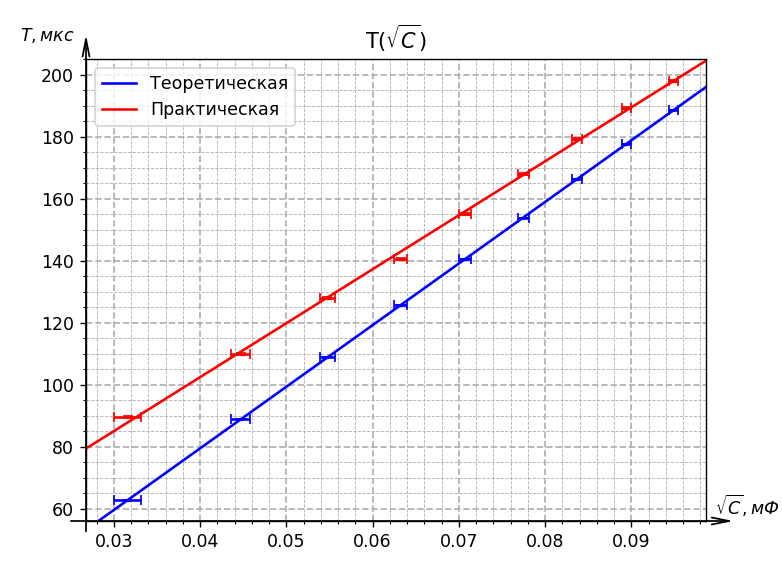
\includegraphics[width=0.8\linewidth]{T(C).png}

\end{figure}

Как видим, прямая практических измерений лежит выше теоретической, это связано в первую очередь с неидеальностью контура, из-за этого период возрастает, так же с тем, что реальная ёмкость цепи несколько больше, чем ёмкость конденсатора.

\begin{table}[h]
        \centering
        \begin{tabular}{|c|c|c|c|c|}
                \hline
                $R_{\text{вн}}$, Ом & $R = R_{\text{вн}} + R_L$, Ом& $\theta = \ln \frac{U_k}{U_{k+1}}$ & $Q = \frac{\pi}{\theta}$ & $\sigma_{Q}$ \\ \hline
                  408.0 & 443.0 & 0.38 & 8.25 & 0.65 \\ \hline
                653.2 & 688.2 & 0.54 & 5.81 & 0.32  \\ \hline
                898.2 & 933.2 & 0.73 & 4.30 & 0.18 \\ \hline
                1143 & 1178 & 0.92 & 3.42 & 0.11 \\ \hline
                1633 & 1668 & 1.27 & 2.46 & 0.06 \\ \hline
        \end{tabular}
        \caption{Декремент затухания свободных колебаний}
\end{table}


Снимем зависимость амплитуды от количества колебаний при разных сопротивлениях контура (данные см. в приложении п. 2). По каждому измерению рассчитаем логарифмический декремент затухания:
\begin{equation}
    \Theta = \frac{1}{n} \cdot \text{ln}(\frac{U_m}{U_{m+n}}).
\end{equation}

Построим график зависимости $1/\Theta^2$ от $1/R_\Sigma ^2$, где $R_\Sigma$ -- суммарное активное сопротивление контура (сопротивление индуктивности измерена в последнем пункте с помощью LCR-измерителя). Получим:

\begin{figure}[h!]
    \centering
    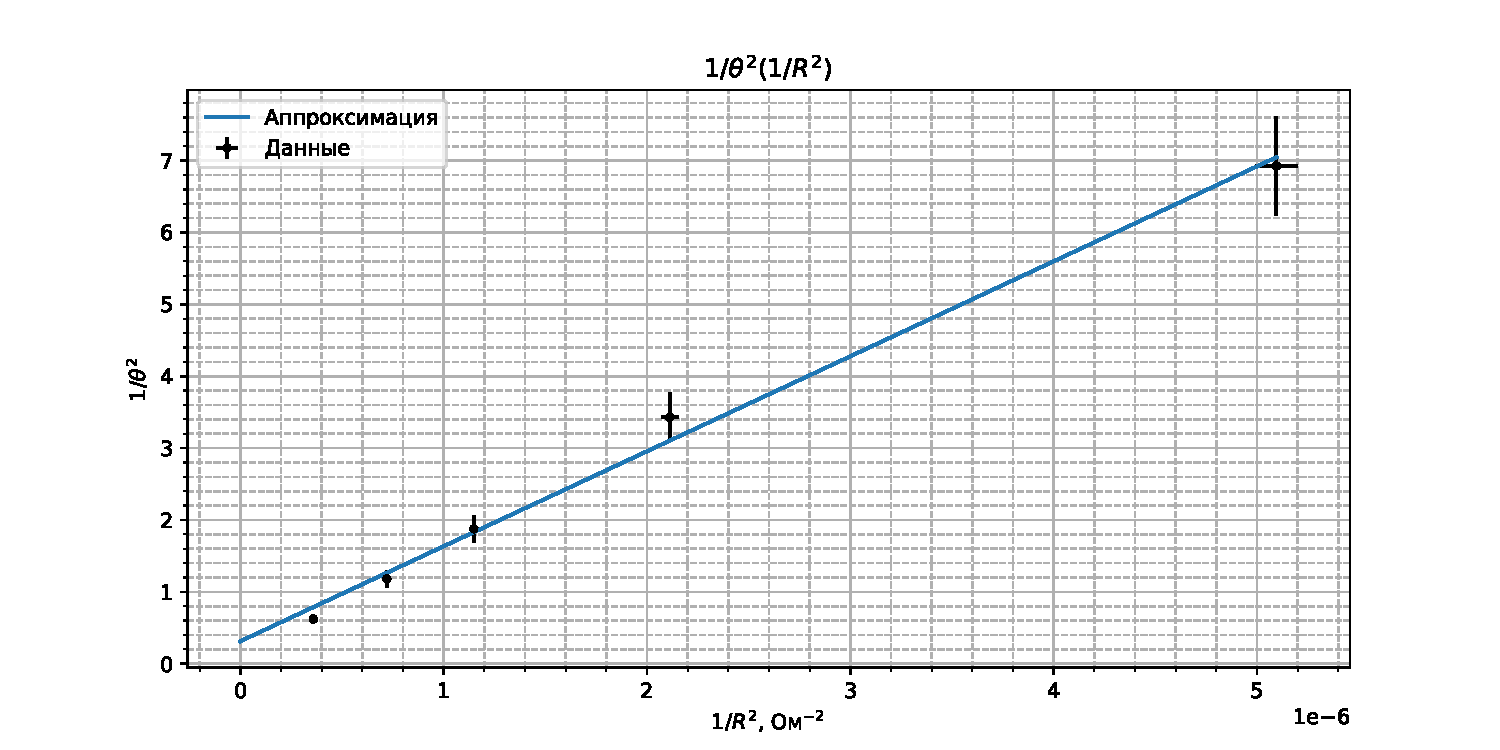
\includegraphics[width=\textwidth]{th(r).pdf}
    \caption{График зависимости логарифмического коэффициента затухания от сопротивления цепи в линеализирующих координатах}
\end{figure}
В ходе измерений невозможно точно установить начало отсчёта амплитуды, из-за чего значения декремента несколько разнятся, в зависимости от того, какая часть сигнала использовалась как источник (положительная или отрицательная), эта проблема частично решается усреднением значений (так как связанное с этим эффектом отклонение близко к погрешности измерений), для этого количество измерений положительной и отрицательной частей совпадают.

По углу наклона рассчитаем $R_\text{кр}$: $R_\text{кр} = 2 \pi \sqrt{\text{tan}(\alpha)} = 6.2 \pm 0.4 \ \text{кОм}.$ Из теории получим: $R_\text{кр} = \sqrt{L/C} = 8.16 \pm 0.07 \ \text{кОм}.$ И посмотрим при каком R на практике происходит переход в апериодический режим:
$R_\text{кр} = 3 \ \text{кОм}.$

Однако точно отличить апериодический режим от быстро затухающего невозможно (нет точного определения), так что будем считать, что следующий режим уже апериодический:
\begin{figure}[h!]
    \centering
    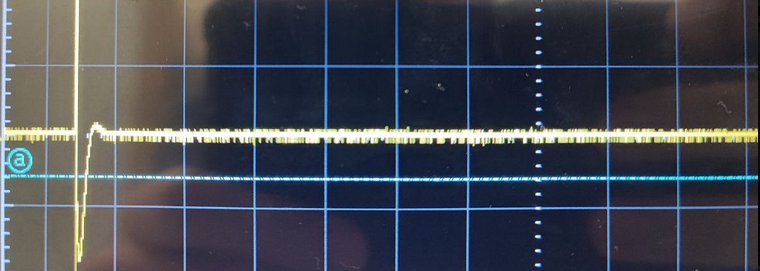
\includegraphics[width=0.8\linewidth]{aperiod.png}
    \caption{Форма сигнала колебаний, которые считаем апериодическими}
\end{figure}
Так же на этом снимке прекрасно видна причина неточного установления начала отсчёта амплитуды.
Снимем спирали на фазовой плоскости, по каждой спирали получим данные о падении амплитуд и так же, как мы делали для предыдущего пункта, рассчитаем декременты затухания и через них получим добротность по формуле:
\begin{equation}
    Q = \pi / \Theta.
\end{equation}

% Please add the following required packages to your document preamble:
% \usepackage[table,xcdraw]{xcolor}
% If you use beamer only pass "xcolor=table" option, i.e. \documentclass[xcolor=table]{beamer}
\begin{table}[h!]
\begin{tabular}{|l|l|l|l|}
\hline
\rowcolor[HTML]{343434}
{\color[HTML]{FFFFFF} $R_\Sigma, \ \text{Ом}$} & {\color[HTML]{FFFFFF} $Q_\text{синус}$} & {\color[HTML]{FFFFFF} $Q_\text{фазовая}$} & {\color[HTML]{FFFFFF} $Q_\text{теоретическая}$} \\ \hline
$ 169.1 \pm 1.0 $                              & $ 18.7 \pm 1.1 $                        & $ 18.0 \pm 0.9 $                          & $ 24.14 \pm 0.25 $                              \\ \hline
$ 309.1 \pm 1.0 $                              & $ 10.8 \pm 0.6 $                        & $ 10.7 \pm 0.3 $                          & $ 13.2 \pm 0.12 $                               \\ \hline
$ 449.1 \pm 1.0 $                              & $ 7.9 \pm 0.4 $                         & $ 7.9 \pm 0.4 $                           & $ 9.09 \pm 0.08 $                               \\ \hline
$ 519.1 \pm 1.0 $                              & $ 6.8 \pm 0.3 $                         & $ 7.0 \pm 0.3 $                           & $ 7.86 \pm 0.07 $                               \\ \hline
$ 589.1 \pm 1.0 $                              & $ 6.8 \pm 0.7 $                         & $ 5.8 \pm 0.3 $                           & $ 6.93 \pm 0.06 $                               \\ \hline
$ 729.1 \pm 1.0 $                              & $ 5.0 \pm 0.3 $                         & $ 4.9 \pm 0.3 $                           & $ 5.6 \pm 0.05 $                                \\ \hline
$ 379.1 \pm 1.0 $                              & $ 9.3 \pm 0.6 $                         & $ 9.2 \pm 0.5 $                           & $ 10.77 \pm 0.09 $                              \\ \hline
$ 659.1 \pm 1.0 $                              & $ 5.6 \pm 0.5 $                         & $ 5.4 \pm 0.3 $                           & $ 6.19 \pm 0.05 $                               \\ \hline
\end{tabular}
\end{table}

Переведём источник сигнала в синусоидальный режим, соберём схему в соответствии с рис. 2. Будем снимать зависимость амплитуды колебаний и разности фаз между генератором и колебаниями в системе от частоты генератора вблизи резонанса (6 кГц) (результаты измерений см. в приложении п.3). Построим АЧХ в нормированных на резонанс координатах $U/U_0$ от $\nu/\nu_0$. Будем аппроксимировать данные точки функцией Лоренца:
$$y = \frac{A}{\sqrt{1-(\frac{x-a}{c})^2}} + s.$$
\begin{figure}[h!]
    \centering
    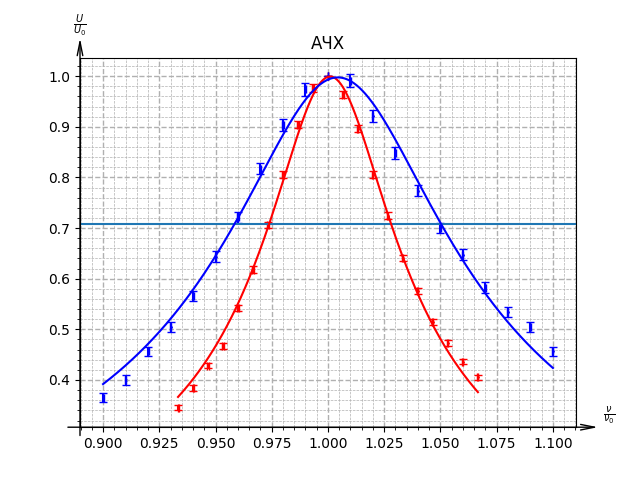
\includegraphics[width=0.8\linewidth]{ACHH.png}
    \caption{Амплитудно-частотная характеристика системы при $R = 440$ Ом -- красная кривая, при $R = 1668$ Ом -- синяя кривая}
\end{figure}

С помощью ширины среза на уровне $1/\sqrt{2}$ получим добротность по формуле:
\begin{equation}
    Q = \frac{\nu_0}{2 \Delta \Omega}
\end{equation}
Ширина резонансной кривой, измеренная на уровне $\frac{A}{\sqrt{2}}$ при сопротивлении магазина 443 Ом равна: $\Delta \Omega_\text{140} = 0,055 \pm 0,005.$
Ширина резонансной кривой, измеренная на уровне $\frac{A}{\sqrt{2}}$ при сопротивлении магазина 1668 Ом равна: $\Delta \Omega_\text{280} = 0,092 \pm 0,005.$
Добротность, рассчитанная с помощью АЧХ, при сопротивлении магазина 140 Ом равна: $\Omega_\text{140} = 8.33\pm 0.69.$
Добротность, рассчитанная с помощью АЧХ, при сопротивлении магазина 280 Ом равна: $\Omega_\text{280} = 2.33 \pm 0.16.$

Построим ФЧХ, для этого пересчитаем $\Delta X$ в разность фаз, для этого воспользуемся формулой:
\begin{equation}
    \Delta \varphi = \frac{1}{\sqrt{LC}} \Delta X.
\end{equation}

Нормируем его по $\pi$, так же измерения при 240 Ом необходимо совместить по фазе (измерялось $\Delta X$ не между ближайшими горбами). Аппроксимировать точки будем с помощью функции: $$y = \frac{\text{arctan}(-a\cdot (x - s))}{\pi} + r.$$ Получим график:

\begin{figure}[h!]
    \centering
    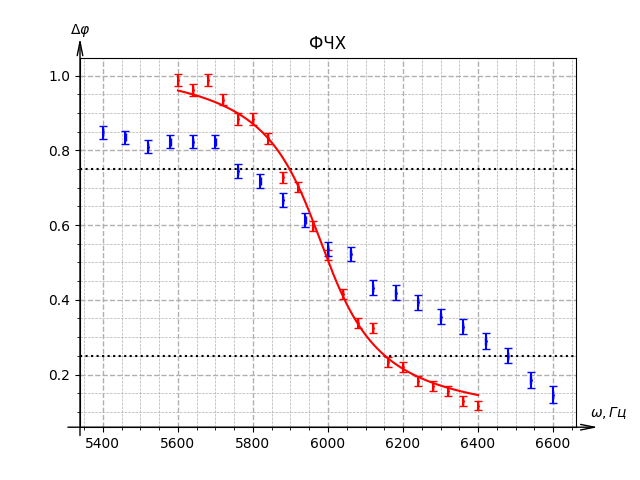
\includegraphics[width=0.8\linewidth]{FCHH.png}
    \caption{Фазо-частная характеристика системы при $R = 440$ Ом -- красная кривая, при $R = 1668$ Ом -- синяя кривая}
\end{figure}

Как видим, по синим точкам не удалось получить искомый вид зависимости, это связано с тем, что нам не хватило области измерений, чтобы застать характерные изгибы нашей функции, так что аппроксимировать к этим точкам смысла нет, уберём их из рассмотрения. Чтобы определить добротность, проведём 2 пунктирные линии на уровнях 0,75 и 0,25. Из нетрудный теоретических соображений можно понять, что через разницу абсцисс этих точек можно определить добротность системы по формуле:
\begin{equation}
    Q = \frac{\nu_0}{\Delta \nu}.
\end{equation}
%Добротность, рассчитанная с помощью ФЧХ, при сопротивлении магазина 140 Ом равна: $Q_\text{ФЧХ} = 43,0 \pm 0,4.$


% Далее переведём генератор в режим испускания цугов и будем снимать показания при установлении колебаний и их спада, будем похожим на пункты 3-4 образом получать данные об изменении амплитуд, через что нетрудно определить добротность по формулам.

% Для установления колебаний:
% \begin{equation}
%     Q = \frac{1}{n} \cdot \text{ln}(\frac{U_0 - U_m}{U_0 - U_{m+n}}).
% \end{equation}

% Для затухания, формула такая же, как и пунктах 3-4:
% \begin{equation}
%     Q = \frac{1}{n} \cdot \text{ln}(\frac{U_m}{U_{m+n}})
% \end{equation}

% Получим следующие добротности:

% Добротность, рассчитанная с помощью логарифмического декремента затухания, при затухании колебаний и сопротивлении магазина 140 Ом равна: $Q_\text{140u} = 16,5 \pm 1,3.$

% Добротность, рассчитанная с помощью логарифмического декремента затухания, при затухании колебаний и сопротивлении магазина 280 Ом равна: $Q_\text{140u} = 10,7 \pm 0,5.$

% Добротность, рассчитанная с помощью логарифмического декремента затухания, при установлении колебаний и сопротивлении магазина 140 Ом равна: $Q_\text{140u} = 17,6 \pm 1,0.$

% Добротность, рассчитанная с помощью логарифмического декремента затухания, при установлении колебаний и сопротивлении магазина 280 Ом равна: $Q_\text{140u} = 10,9 \pm 1,0.$

% Пронаблюдаем картину биений:
% \begin{figure}[h!]
%     \centering
%     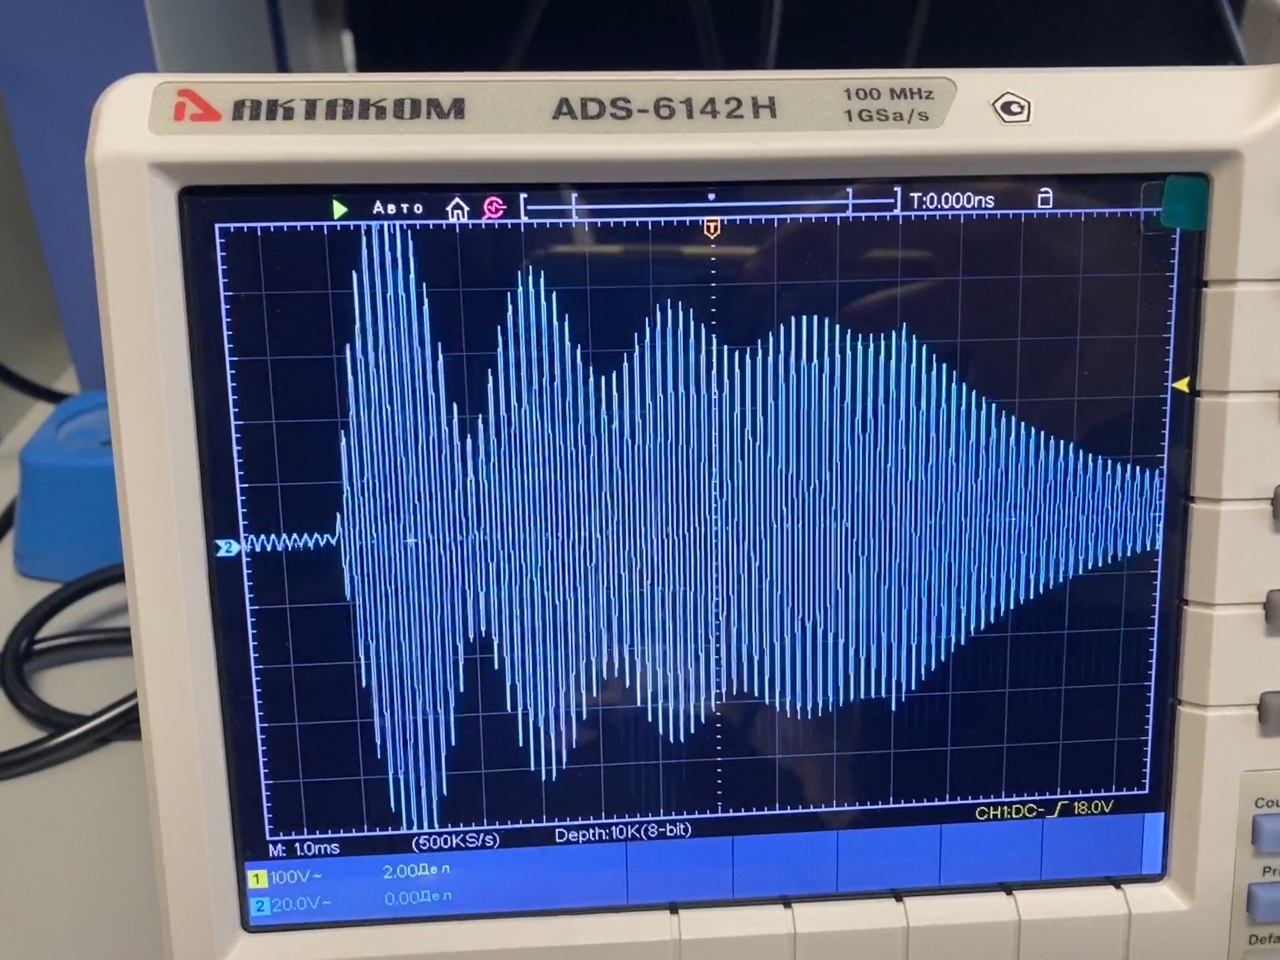
\includegraphics[width=0.8\linewidth]{bien.jpg}
%     \caption{Картина наблюдаемых биений}
% \end{figure}

% На данной картине биений мы можем наблюдать два участка, первый -- установление вынужденных колебаний, такой режим происходит из-за того, что разница частот генератора и колебательной системы мала по сравнению с характерным временем установления постоянного режима вынужденных колебаний, через некоторое время после установления произойдёт затухание амплитуды колебаний, связанное с нарастающей разностью фаз между генератором и системой. Через некоторый промежуток времени такая картина повторится.


\section{Погрешности измерений}
В ходе вычислений погрешностей в основном использовалась классическая модель погрешности:
$$ \sigma = \sqrt{(\sigma_\text{случ})^2 + (\sigma_\text{систем})^2}.$$

Для обычных математических операций использовалась модель о сумме квадратов относительных погрешностей величин, входящих в формулу:
$$ \varepsilon = \sqrt{\varepsilon_1^2 + \varepsilon_2^2}.$$

Для обработки случайных погрешностей при повторных измерениях использовалась следующая модель:
$$\sigma = \frac{1}{\sqrt{n}} \cdot \sqrt{\sum_i(x_i - x_\text{ср})^2}.$$

% Аппроксимация производилась с помощью метода $curve_fit$ из библиотеки SciPy, соответственно модель вычисления случайной погрешности при аппроксимации Хи-квадрат. За более детальным описанием можно обратиться к исполняемому коду.

%\newpage
\section{Вывод}
\begin{enumerate}
    \item В ходе сравнения зависимости с теоретической была обнаружена некоторая небольшая ёмкость колебательной системы (исключая магазин ёмкостей), которая смещает зависимость $T(C)$ на некоторую константу, однако, достаточно мала, чтобы изменить характер зависимости (изменений установить не удалось).
    % \begin{figure}[h!]
    % \centering
    % 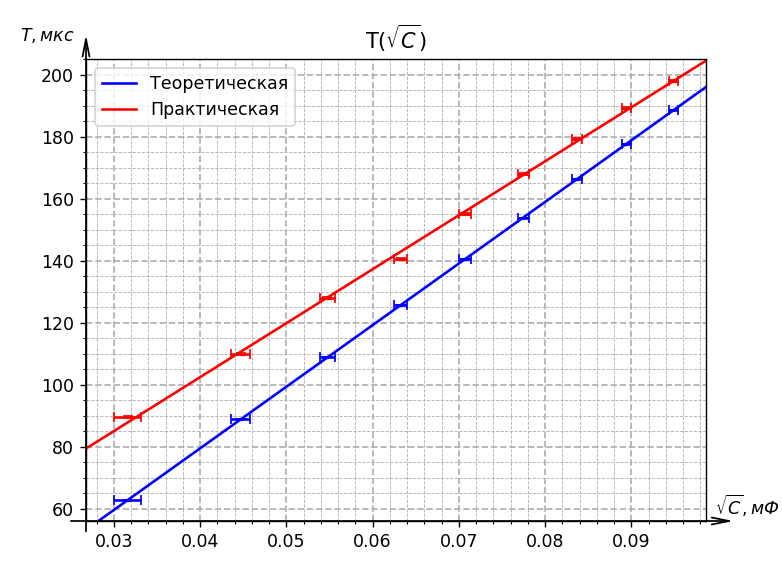
\includegraphics[width=0.6\linewidth]{T(C).png}
    % \caption{График зависимости периода собственных колебаний от корня из ёмкости системы}
    % \end{figure}
    \item Удалось снять зависимость логарифмического декремента затухания от активного сопротивления цепи (погрешность составила порядка $5\%$), основной причиной такой погрешности послужили наводки, которые <<размазывали сигнал>>, особенно на пиках амплитуд, делая невозможным поддерживать точность на уровне точности приборов.
    % \begin{figure}[h!]
    % \centering
    % 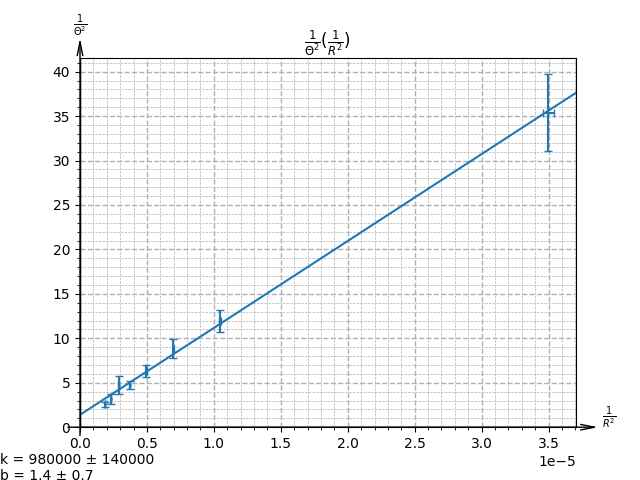
\includegraphics[width=0.6\linewidth]{th(r).png}
    % \caption{График зависимости логарифмического коэффициента затухания от сопротивления цепи в линеализирующих координатах}
    % \end{figure}
    %\newpage
    \item Определили критическое сопротивление, при котором характер колебаний меняется на апериодический, тремя способами: теоретическим $R_\text{кр} = 8,16 \pm 0,07 \ \text{кОм},$ по наклону графика зависимости логарифмического декремента затухания от сопротивления цепи $R_\text{кр} = 6,2 \pm 0,4 \ \text{кОм},$ с помощью наблюдением за картиной колебаний $R_\text{кр} = 3 \ \text{кОм}.$ Как видим, значения довольно сильно отличаются, это связано с неточностью $R_\text{кр}$ по своей природе.

    \item Были сняты АЧХ и ФЧХ для вынужденных колебаний в цепи, проведена аппроксимация соответствующих теоретических зависимостей к экспериментальным точкам, функции из теории хорошо ложатся на точки, однако при этих измерениях возникли ещё большие наводки, сделали случайную погрешность кратно больше системной ($\sigma_\text{случ} \sim 7 \sigma_\text{сист}$), однако из-за аппроксимации они не имею большого вклада в итоговые результаты.
    % \begin{figure}[h!]
    % \centering
    % 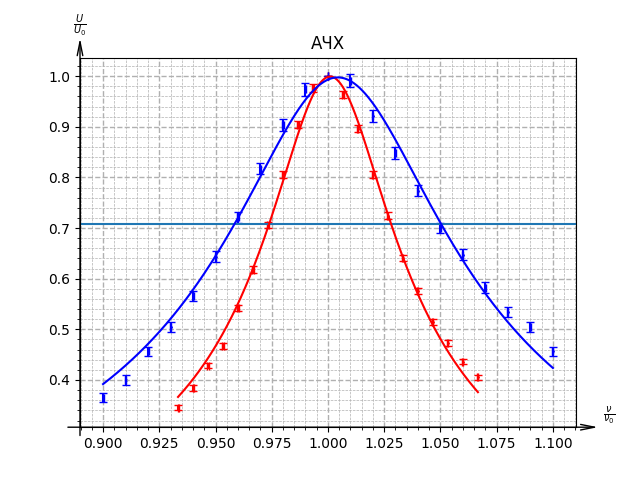
\includegraphics[width=0.6\linewidth]{ACHH.png}
    % \caption{Амплитудно-частотная характеристика системы при $R = 140$ Ом -- красная кривая, при $R = 280$ Ом -- синяя кривая}
    % \end{figure}
    % \begin{figure}[h!]
    % \centering
    % 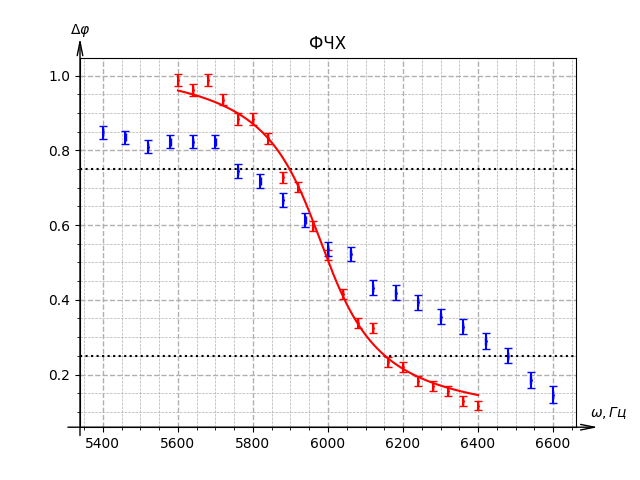
\includegraphics[width=0.6\linewidth]{FCHH.png}
    % \caption{Фазо-частная характеристика системы при $R = 140$ Ом -- красная кривая, при $R = 280$ Ом -- синяя кривая}
    % \end{figure}

    \item Удалось определить логарифмические декременты затухания по установлению и затуханию вынужденных колебаний, получены значения декремента для двух значений сопротивления магазина:

    при $R = 140 \ \text{Ом}$ $\Theta_\text{затух} = 0.19 \pm 0.015;$ $\Theta_\text{устан} = 0.179 \pm 0.01$,

    при $R = 280 \ \text{Ом}$ $\Theta_\text{затух} = 0.293 \pm 0.013;$ $\Theta_\text{устан} = 0.29 \pm 0.03$.

    Как видим, значения хорошо совпадают в пределах погрешностей.

    \item Удалось понять, что такая картина биений получается из-за комбинации установления вынужденных колебаний, и только после этого классических биений. Однако на установке посылались цуги довольно большой длины, так что последняя часть данной картины была уже простыми затухающими колебаниями.
    % \begin{figure}[h!]
    % \centering
    % 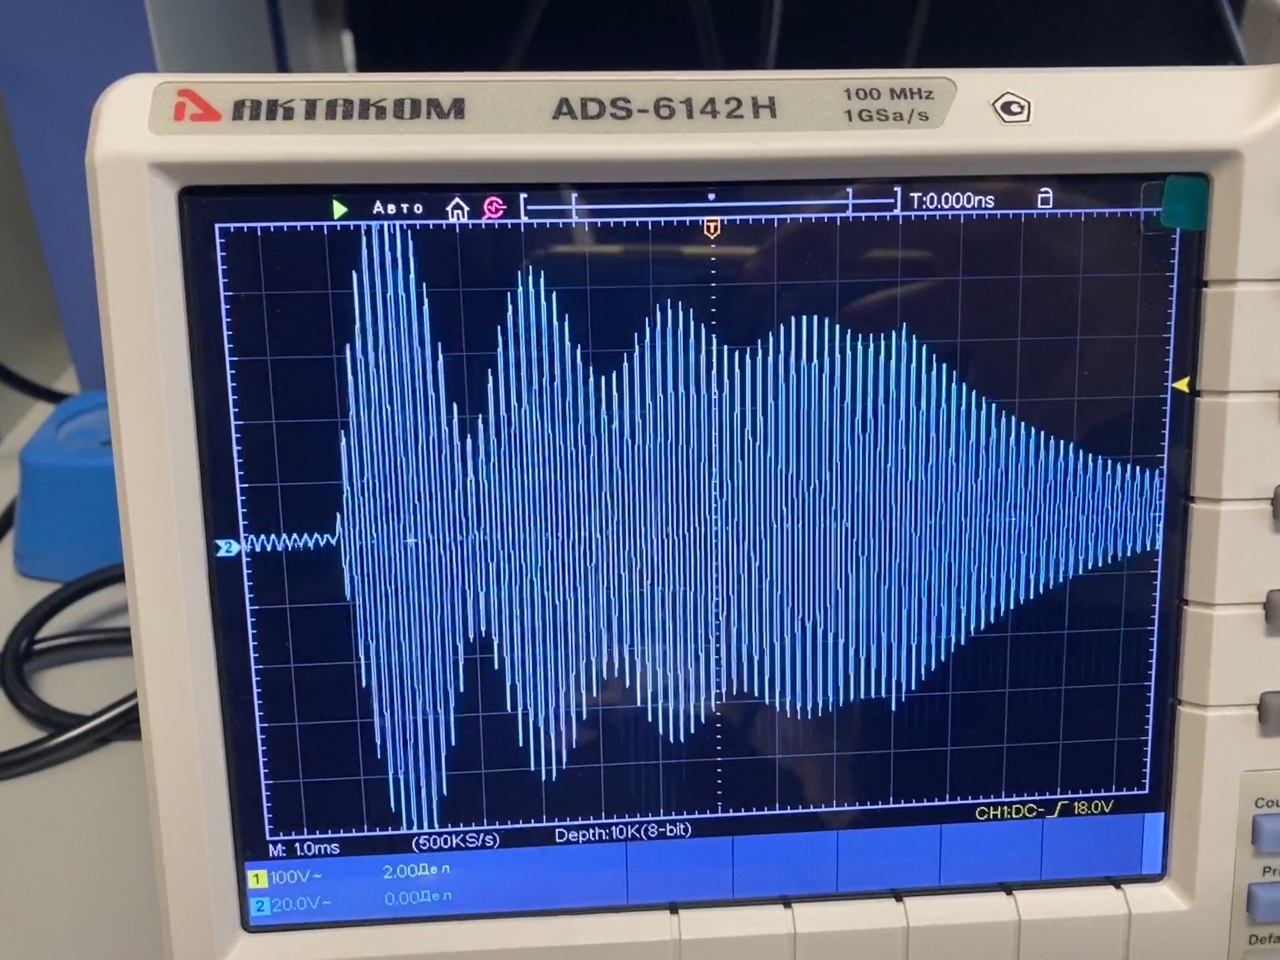
\includegraphics[width=0.8\linewidth]{bien.jpg}
    % \caption{Картина наблюдаемых биений}
    % \end{figure}

    \item Результаты измерения добротности вышеизложенными способами изложены в таблице:

    \begin{table}[h]
        \centering
        \begin{tabular}{|c|c|c|c|c|c|}
                \hline
                $R$, Ом & $f(L, C, R)$ & $f(\theta)$ & Фаз. спираль & АЧХ & ФЧХ \\ \hline
                443 & $9.20 \pm 0.10$ & $8.25 \pm 0,65$& $8.20 \pm 0.86$ & $8.33 \pm 0.69$ & $8.70\pm 0.76$ \\
                & $(1\%)$ & $(8\%)$ & $(10\%)$ & $(8\%)$ & $(9\%)$  \\ \hline
                1668 & $2.40 \pm 0.01$ & $ 2.46 \pm 0.06$ & $ 2.35 \pm 0.18$ & $2.33 \pm 0.16  $ & $2.41 \pm 0.17 $ \\
                & $(0.3 \%)$ & $(2\%) $ & $(8\%) $ & $(7 \%) $ & $(7 \%) $ \\ \hline
        \end{tabular}
    \end{table}

    Как видим, почти все добротности хорошо совпали (максимальное различие $1 \sigma$), однако добротность ФЧХ сильно выбивается из результатов, вероятно, где-то потерян коэффициент, так же, как и ожидалось, теоретическая добротность выше практической, что связано с лишними сопротивлениями в реальной цепи.


\end{enumerate}


\end{document}